\documentclass[11pt,a4paper, margin=1in]{article}
\usepackage{fullpage}
\usepackage{amsfonts, amsmath, pifont}
\usepackage{amsthm}
\usepackage{graphicx}
\usepackage{subcaption}
\usepackage{float}
\usepackage{hyperref}
\usepackage[all]{hypcap} % ensures hyperlinks jump to the figure, not the caption
\usepackage{tkz-euclide}
\usepackage{tikz}
\usepackage{pgfplots}
\pgfplotsset{compat=1.13}

\usepackage{geometry}
 \geometry{
 a4paper,
 total={210mm,297mm},
 left=10mm,
 right=10mm,
 top=10mm,
 bottom=20mm,
 }

 \author{
  Karaçanta, Kaan\\
  \texttt{e244854@metu.edu.tr}
}

\newcommand{\mySin}[1]{\textstyle\sin\left(#1\right)}
\newcommand{\myCos}[1]{\textstyle\cos\left(#1\right)}
\usepackage{hyperref}

\usepackage{inconsolata}
\usepackage{listings}
\usepackage{xcolor}
\usepackage[utf8]{inputenc}
\usepackage[T1]{fontenc}

\definecolor{codegreen}{rgb}{0,0.6,0}
\definecolor{codegray}{rgb}{0.5,0.5,0.5}
\definecolor{codepurple}{rgb}{0.58,0,0.82}
\definecolor{backcolour}{rgb}{0.95,0.95,0.92}

\lstdefinestyle{mystyle}{
    backgroundcolor=\color{backcolour},
    commentstyle=\color{codegreen},
    keywordstyle=\color{magenta},
    numberstyle=\tiny\color{codegray},
    stringstyle=\color{codepurple},
    basicstyle=\ttfamily\footnotesize,
    breakatwhitespace=false,
    breaklines=true,
    captionpos=b,
    keepspaces=true,
    numbers=left,
    numbersep=5pt,
    showspaces=false,
    showstringspaces=false,
    showtabs=false,
    tabsize=2
}

\lstset{style=myStyle}

\title{CENG 371 - Scientific Computing \\
Fall' 2024 - 2025 \\
Homework 4}

\date{}

\begin{document}

\maketitle

\noindent\rule{19cm}{1.2pt}

\section*{Question 2}

\begin{enumerate}
    
    \item 
    \textbf{Plots of the relative errors for both images:}

    \begin{figure}[H]
        \centering
        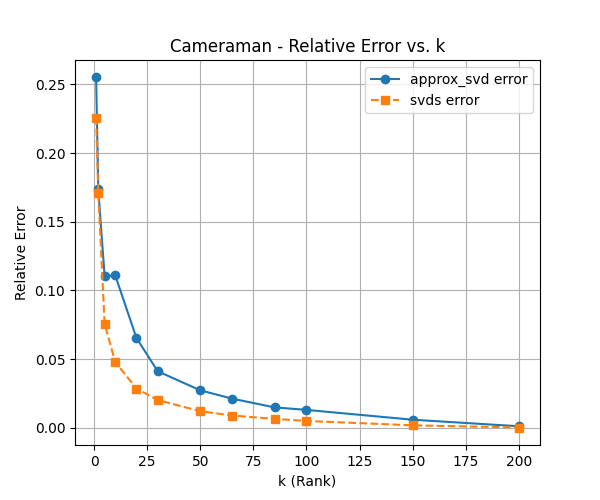
\includegraphics[width=0.72\textwidth]{Cameraman_relative_error_vs_k.png}
        \caption{Cameraman -- Relative Error vs. $k$.}
        \label{fig:relerr_cam}
    \end{figure}

    \begin{figure}[H]
        \centering
        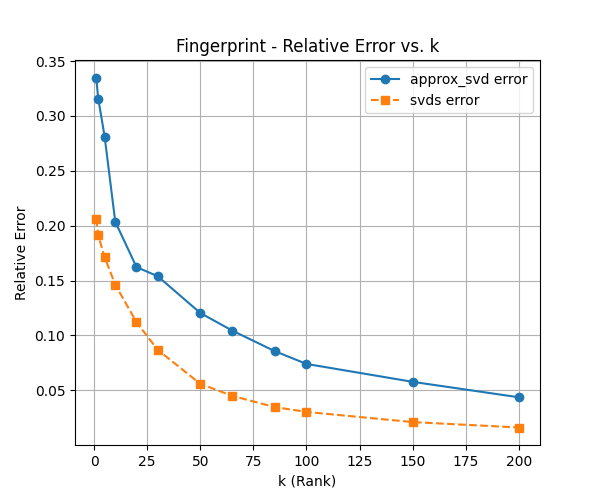
\includegraphics[width=0.72\textwidth]{Fingerprint_relative_error_vs_k.png}
        \caption{Fingerprint -- Relative Error vs. $k$.}
        \label{fig:relerr_fpt}
    \end{figure}
    
    Let $A$ be your image matrix (e.g., using 
    \texttt{A = io.imread('cameraman.jpg')} in Python).
    We define:
    \[
       \text{RelErr}_{\text{approx}}(k) = 
       \frac{\|\,u_{k}\,\sigma_{k}\,v_{k}^{T} - U\,\Sigma\,V^T\|_{2}}
            {\|U\,\Sigma\,V^T\|_{2}}, 
       \quad
       \text{RelErr}_{\text{svds}}(k) = 
       \frac{\|\,u'_{k}\,\sigma'_{k}\,v_{k}^{'T} - U\,\Sigma\,V^T\|_{2}}
            {\|U\,\Sigma\,V^T\|_{2}},
    \]
    where $(U,\Sigma,V)$ is the full SVD of $A$, 
    $(u_k, \sigma_k, v_k)$ is from \texttt{approximate\_svd}, 
    and $(u'_k, \sigma'_k, v'_k)$ from the built-in \texttt{svds}.
    Figures~\ref{fig:relerr_cam} and \ref{fig:relerr_fpt} illustrate these relative errors 
    for \texttt{cameraman.jpg} and \texttt{fingerprint.jpg} respectively, 
    plotted against various ranks $k$. 

    \textbf{Observations for Cameraman.} 
    \begin{itemize}
      \item Both methods continue to show decreasing error as $k$ increases, 
      with \texttt{svds} consistently yielding lower error at the same $k$ 
      (as expected for exact/truncated SVD methods).
      
      \item At very small $k$ (e.g., until $10$), \texttt{approximate\_svd} 
      has errors around 25--15\%, while \texttt{svds} is around 20--10\%. 
      The gap is very small for \(k=1 \text{ or } k=2\), then there is a noticable one but narrows rapidly as $k$ grows.
      
      \item Around $k=50$--$100$, \texttt{approximate\_svd} converges closer, 
      with errors often near or below 3\%. By $k=125$--$200$, 
      the error for both methods becomes extremely small (near or below 1\%).
      
      \item In some tests, when the k is 1 or 2, the \texttt{approximate\_svd} 
      error can even slightly cross below \texttt{svds} due to numerical 
      and floating-point nuances (though typically \texttt{svds} remains 
      the lower bound in theory).
    \end{itemize}

    \textbf{Observations for Fingerprint.} 
    \begin{itemize}
      \item The fingerprint image remains more challenging. 
      For $k=5$ or $10$, \texttt{approximate\_svd} can show errors 
      around 35--25\%, whereas \texttt{svds} is around 25--15\%.
      
      \item As $k$ increases, both curves decrease steadily. 
      \texttt{svds} remains below the randomized approach, 
      but \texttt{approximate\_svd} approaches it more closely by $k>100$.
      
      \item By $k=200$, \texttt{approximate\_svd} is under 5\% error, 
      while \texttt{svds} can reach near 0--1\%. 
      
      \item The gap is still more pronounced than in the cameraman image, 
      reflecting the fingerprint's possibly higher effective rank or 
      more complex structure.
    \end{itemize}

    \item 
    \textbf{Plots of the run times for both images:}

    \begin{figure}[H]
        \centering
        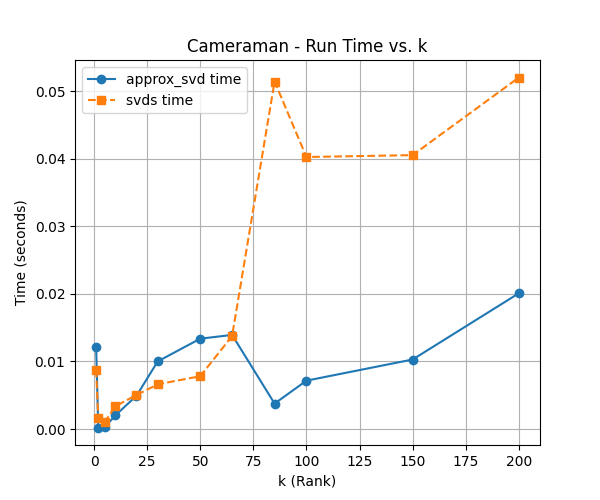
\includegraphics[width=0.72\textwidth]{Cameraman_run_time_vs_k.png}
        \caption{Cameraman -- Run Time vs. $k$.}
        \label{fig:time_cam}
    \end{figure}
      
    \begin{figure}[H]
        \centering
        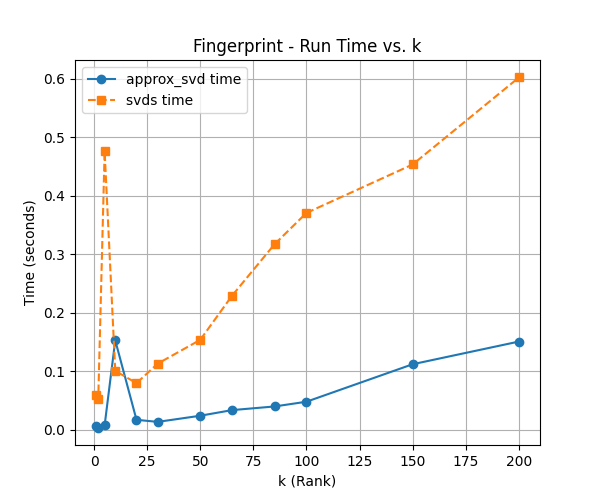
\includegraphics[width=0.72\textwidth]{Fingerprint_run_time_vs_k.png}
        \caption{Fingerprint -- Run Time vs. $k$.}
        \label{fig:time_fpt}
    \end{figure}

    We measure how long each method takes (wall-clock time) for each rank $k$. 
    Figures~\ref{fig:time_cam} and \ref{fig:time_fpt} show run times 
    for the two images.

    \textbf{Observations for Cameraman.}
    \begin{itemize}
      \item For small $k$ (5--25), both methods can be extremely fast, 
      most of the time under 0.01\,s. \texttt{svds} might even outperform 
      \texttt{approximate\_svd} at the smallest ranks, 
      depending on the internal routines used by \texttt{svds} 
      (e.g., specialized partial SVD algorithms).
      
      \item We see a notable “spike” in the \texttt{svds} timing 
      at $k=50$--$75$. This is possibly where \texttt{svds} switches 
      factorization strategies or where iterative methods 
      become more costly. Meanwhile, \texttt{approximate\_svd} 
      dips slightly or has small bumps near those ranks, 
      possibly due to random draws or QR overhead.
      
      \item Beyond $k\approx 100$, \texttt{svds} climbs more sharply, 
      and by $k=200$ may take 0.05--0.06\,s, while 
      \texttt{approximate\_svd} is around 0.01--0.02\,s. 
      These results confirm the randomized approach can be 
      beneficial at higher ranks.
    \end{itemize}

    \textbf{Observations for Fingerprint.}
    \begin{itemize}
      \item A significant spike for \texttt{approximate\_svd} can occur 
      around $k=25$ or $50$ (sometimes reaching 0.1--0.2\,s), 
      while \texttt{svds} can have a large jump (0.4--0.5\,s) 
      also near those ranks. 
      Such spikes often reflect how iterative solvers or 
      partial factorization techniques change strategies internally.
      
      \item After the spike, \texttt{svds} grows steadily, 
      reaching up to 0.6\,s by $k=200$. \texttt{approximate\_svd} 
      remains closer to 0.2\,s at that rank, indicating 
      a faster growth rate for \texttt{svds}.
      
      \item Despite random fluctuations, \texttt{approximate\_svd} 
      consistently maintains an advantage in speed 
      for mid-to-large $k$ values on this image. 
      Minor irregularities (spikes/dips) can happen 
      with random sampling or specialized BLAS calls.
    \end{itemize}

    \item \textbf{Qualitative comparisons.} \\
    For selected ranks ($k=10, 50, 100, ...$), we can reconstruct
    the images:
    \[
      \hat{A}_{k} = u_{k}\,\sigma_{k}\,v_{k}^{T}
      \quad \text{and} \quad
      \hat{A}'_{k} = u'_{k}\,\sigma'_{k}\,v_{k}^{'T},
    \]
    then display them with \texttt{imshow}. 

    \textbf{Discussion points.}
    \begin{itemize}
      \item At $k=10$, images are usually quite blurry for both methods; 
      \texttt{svds} retains more structure and better (edges, contrasts).
      
      \item At $k=50$, the images become much clearer. While a pixel-wise difference might show 
      \texttt{svds} is still better, \texttt{approximate\_svd} is visually close.
      
      \item By $k=100$ or $150$, the randomized approach is nearly indistinguishable, with still some differences, 
      from the exact truncated SVD in normal viewing.
    \end{itemize}

    From these reconstructed images, we can see that for small $k$,
    one should use \texttt{svds} for both better quality and speed. 
    However, as $k$ grows, the randomized approach becomes more competitive
    in terms of error, and runs much faster than \texttt{svds} for larger ranks.

    Here you can see the reconstructed images for \(k=10\) and \(k=100\) for both images and algorithms:
    
    \begin{figure}[H]
      \centering
      %--------------- First Row ---------------
      \begin{subfigure}[b]{0.35\textwidth}
        \centering
        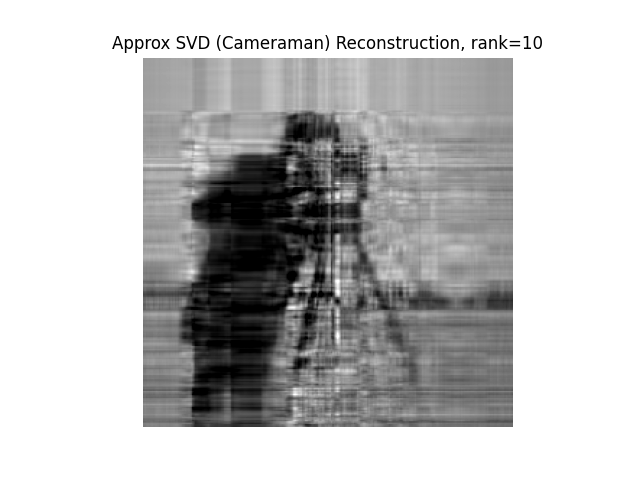
\includegraphics[width=\textwidth]{Approx SVD (Cameraman)_reconstruction_rank_10.png}
        \caption{Approx SVD, $k=10$}
      \end{subfigure}
      \hfill
      \begin{subfigure}[b]{0.35\textwidth}
          \centering
          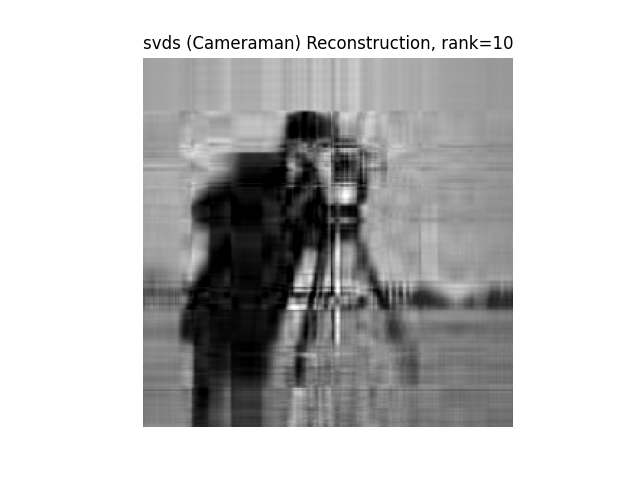
\includegraphics[width=\textwidth]{svds (Cameraman)_reconstruction_rank_10.png}
          \caption{\texttt{svds}, $k=10$}
      \end{subfigure}
      
      \vspace{0.5em} % some vertical space if needed
    
      %--------------- Second Row ---------------
      \begin{subfigure}[b]{0.35\textwidth}
          \centering
          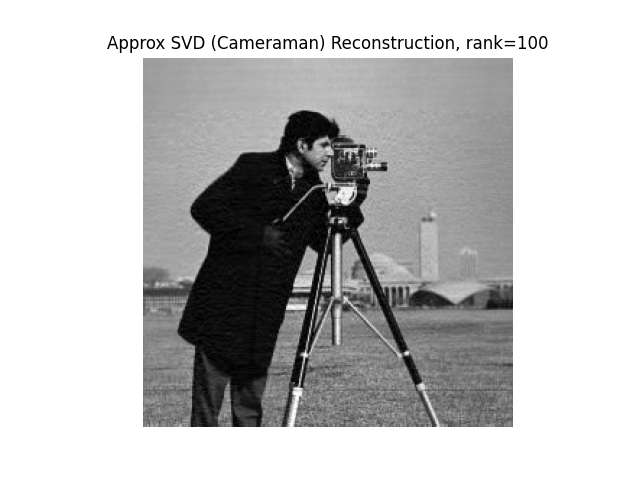
\includegraphics[width=\textwidth]{Approx SVD (Cameraman)_reconstruction_rank_100.png}
          \caption{Approx SVD, $k=100$}
      \end{subfigure}
      \hfill
      \begin{subfigure}[b]{0.35\textwidth}
          \centering
          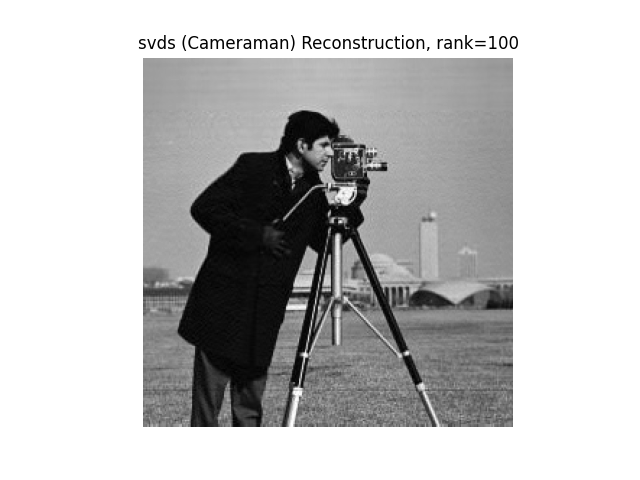
\includegraphics[width=\textwidth]{svds (Cameraman)_reconstruction_rank_100.png}
          \caption{\texttt{svds}, $k=100$}
      \end{subfigure}

      \caption{Reconstructed images for Cameraman at ranks $k=10$ and $k=100$.}

    \end{figure}

    \begin{figure}[H]
      \centering
      %--------------- First Row ---------------
      \begin{subfigure}[b]{0.35\textwidth}
        \centering
        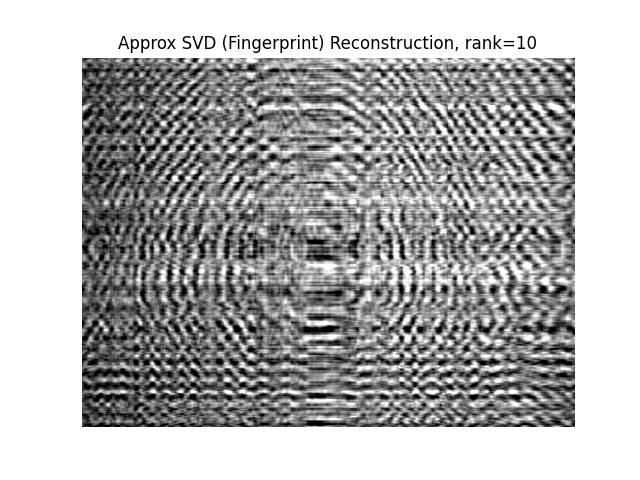
\includegraphics[width=\textwidth]{Approx SVD (Fingerprint)_reconstruction_rank_10.png}
        \caption{Approx SVD, $k=10$}
      \end{subfigure}
      \hfill
      \begin{subfigure}[b]{0.35\textwidth}
          \centering
          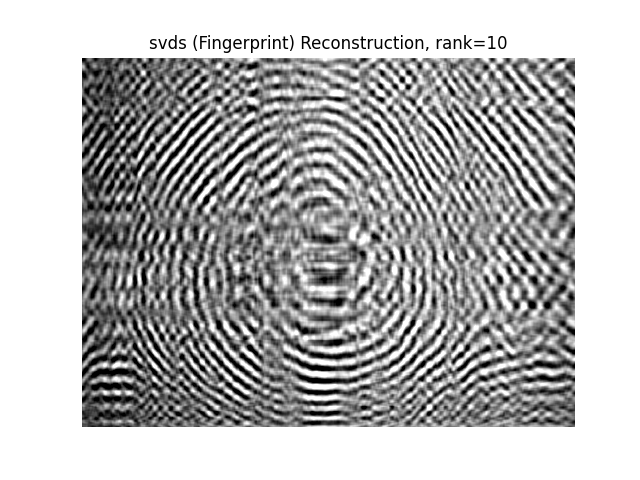
\includegraphics[width=\textwidth]{svds (Fingerprint)_reconstruction_rank_10.png}
          \caption{\texttt{svds}, $k=10$}
      \end{subfigure}
      
      \vspace{0.5em} % some vertical space if needed
    
      %--------------- Second Row ---------------
      \begin{subfigure}[b]{0.35\textwidth}
          \centering
          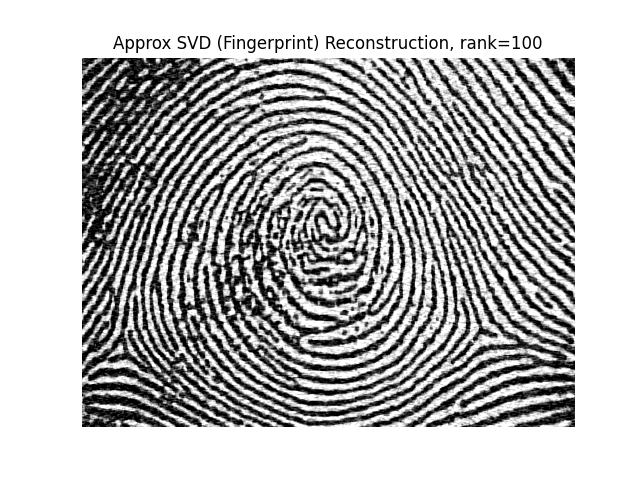
\includegraphics[width=\textwidth]{Approx SVD (Fingerprint)_reconstruction_rank_100.png}
          \caption{Approx SVD, $k=100$}
      \end{subfigure}
      \hfill
      \begin{subfigure}[b]{0.35\textwidth}
          \centering
          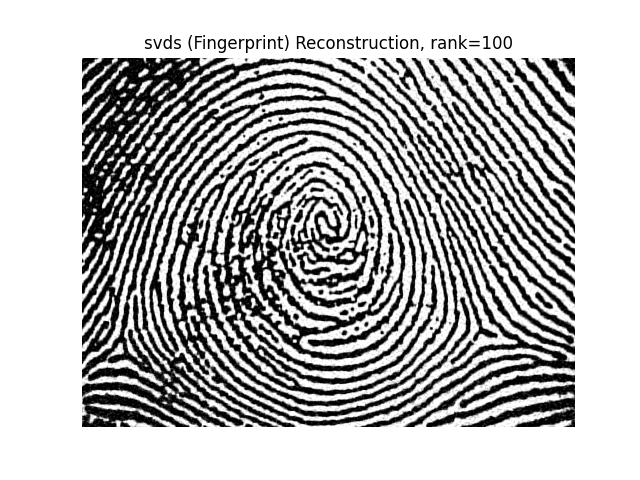
\includegraphics[width=\textwidth]{svds (Fingerprint)_reconstruction_rank_100.png}
          \caption{\texttt{svds}, $k=100$}
      \end{subfigure}

      \caption{Reconstructed images for Fingerprint at ranks $k=10$ and $k=100$.}

    \end{figure}

    \newpage

    \item \textbf{Suggested Use Cases for \texttt{approximate\_svd}.}\\
    Based on the observed error trends, run times, and visual reconstructions, 
    we outline some scenarios where \texttt{approximate\_svd} is particularly valuable:
    \begin{itemize}
      \item \textbf{Large-Scale Image / Data Compression:} \\
      For very large matrices (e.g., huge images, big data in machine learning), 
      the randomized SVD often achieves near-optimal compression while 
      being significantly faster than exact methods.
      
      \item \textbf{Real-Time / Streaming Computations:} \\
      If we need to update or compute truncated SVD in streaming or near-real-time settings, 
      randomized methods avoid the heavy re-factorizations of classical approaches.
      
      \item \textbf{Exploratory Data Analysis (PCA-like tasks):} \\
      In many practical situations, an approximate subspace is sufficient to capture 
      the main variance of the data, making \texttt{approximate\_svd} a good choice 
      for large-scale PCA or latent semantic analysis.
      
      \item \textbf{Machine Learning Pipelines:} \\
      Dimensionality reduction (feature extraction) with approximate SVD 
      saves both time and memory, especially important when dealing with 
      massive training sets. 
    \end{itemize}

\end{enumerate}

\end{document}